% Standard LaTeX document template
%  BE SURE TO PROCESS DOCUMENT TWICE IF IT CONTAINS CROSS-REFERENCES!

\documentclass[12pt]{article}
\usepackage[round]{natbib} %allow to set the bibliography style and
% import the bibliography file. See Bibliography management with
% natbib for more information on
% https://www.sharelatex.com/learn/Bibliography_management_with_natbib.
% See the reference sheet for natbib on
% http://merkel.zoneo.net/Latex/natbib.php.
% Several .bst files can be
% downloaded from http://kinglab.eeb.lsa.umich.edu/pub/biblios/bst/

\usepackage{graphicx,epsfig}
\usepackage{amssymb,amsmath,amsfonts,bm,color,supertabular,longtable,multirow}
\usepackage[colorlinks=true,linkcolor=black,citecolor=black,urlcolor=black]{hyperref}

\setlength{\oddsidemargin}{0in} % left margin, odd pages
\setlength{\evensidemargin}{0in} % left margin, even pages
\setlength{\textwidth}{6.5in} % widtth of text on page
\setlength{\topmargin}{-.3in} % add to default 1 in
\setlength{\headsep}{0in}     % add to default 25pt
\setlength{\textheight}{8.7in}  % height of text on page
\setlength{\parskip}{.1in}            % vertical space between paragraphs
\setcounter{tocdepth}{2}

%\setlength{\parindent}{0in}            % amount of indentation of paragraph


%  newcommands -- more newcommands used in the document.
%  not just in the preamble

\newcommand{\Var}{\mbox{Var}}
\newcommand{\Cov}{\mbox{Cov}}
\newcommand{\E}{\mbox{E}}
\newcommand{\ubeta}{\mbox{\boldmath$\beta$}}
% Independence symbol
\newcommand\independent{\protect\mathpalette{\protect\independenT}{\perp}}
\def\independenT#1#2{\mathrel{\rlap{$#1#2$}\mkern2mu{#1#2}}}


\title{STAT 501 Case Study Assignment} 
\author{Quan Zhao\\
School of Mathematics and Statistics\\ Victoria University of Wellington, New Zealand} 
%\date{}  % Add \date{} to make a blank date.


%  main body of document

\begin{document}

% Titlepage
\maketitle

\begin{abstract}
  This course provides students with an opportunity to develop their
  research skills in Mathematics and Statistics, including use of
  library resources, constructing literature reviews, developing
  research questions, writing research proposals, and developing
  skills in oral presentation. The template file gives an introduction
  to LaTeX,
\end{abstract}


% Table of Contents
\tableofcontents


\setlength{\baselineskip}{0.25in} % min space from bottom of one line

                                 % to top of next in a paragraph

                                 % place after \begin{document}



\newpage  % start from a new page
\section{Introduction}

\label{s.intro}

Context and background information.
\cite{Liu05}

\section{Objectives and Scope}

Specific objectives of the statistical consultation.
Scope of the analysis including what is and is not covered.

% \section{Methodology}

% Overview of the statistical methods used.
% Software and tools used for analysis.

\section{Data Description}

Sources of data.
Description of variables.
Data collection methods.
Data quality and validation procedures.

\subsection{Citizen variables (Micheal)}

% \subsection{Registretion (Felix)}

\subsection{Citizen Registration Analysis (Felix)}

\subsubsection{Start end registrations}
The \textit{start end registrations} table aggregates data for each registration type of citizens. 
Despite the table containing 1048575 rows, a significant majority (1047272 rows) have their 'Type' set as "nan", indicating that these citizens have not specified a registration Type.

Only 357 unique citizens have defined a registration type. 
Fig~\ref{fig:countoftypes}

The distribution of the count of citizens against the number of types selected by them is illustrated in Fig~\ref{fig:howmanytypes}.

\begin{figure}[h]
\centering
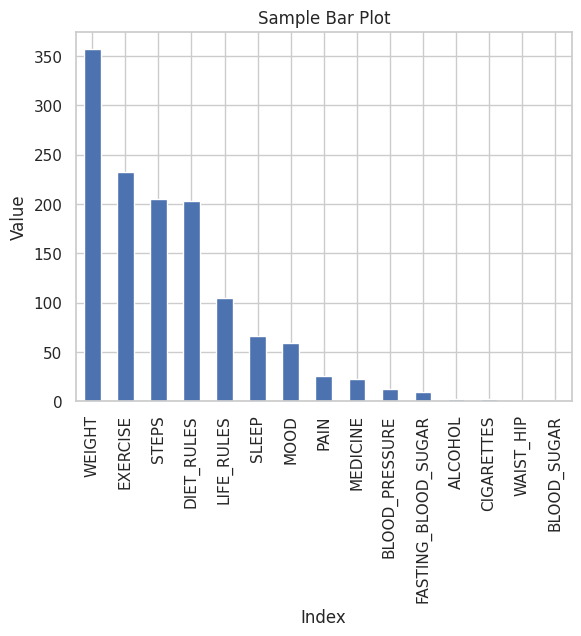
\includegraphics[width=0.7\linewidth]{images/reg_types.png}
\caption{Count of types}
\label{fig:countoftypes}
\end{figure}

\begin{figure}[h]
\centering
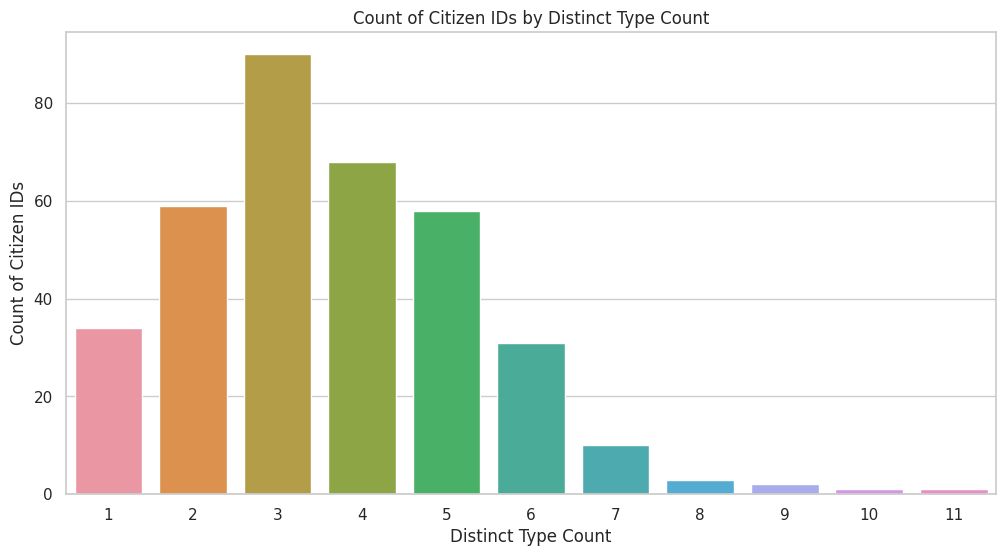
\includegraphics[width=0.7\linewidth]{images/start_end_reg_count.png}
\caption{How many citizens select how many types in start\_end\_registrations}
\label{fig:howmanytypes}
\end{figure}

\subsubsection{Registrations per Goal}
The \textit{registrations per goal} table aggregates registration data by the goal of each registration type for citizens. 

Notably, a single registration type can be associated with multiple goals. There are 362 unique citizens with registration types in both the \textit{registrations per goal} and \textit{goal and registration} tables, differing from the distribution in \textit{start\_end\_registrations}.

\subsubsection{Goal and Registration}
The \textit{goal and registration} table provides detailed registration data for each type and its associated goals for citizens.

\subsubsection{Missing Citizens in Start end registrations}
Upon analysis, it was discovered that four citizens, namely 831841, 909811, 955121, and 1022212, were absent in the \textit{start end registration} table but present in both the \textit{registrations per goal} and \textit{goal and registration} tables.

\subsubsection{Table Selection for Aggregation at the Citizen Level}
The \textit{Start end registrations} table appears to be the most suitable for representing citizen registration activities since it is already aggregated at the registration type level, although, it lacks information on four citizens and excludes the "EXERCISE" category. because of, the \textit{registrations per goal} table detailed goal-wise data for each registration type might result in a substantial aggregation workload. The \textit{goal and registration} table's data is deemed too intricate and is thus not considered for this phase.

For a more comprehensive representation of citizen registration activities, 
We aggregated in registration type level for each citizen based on "valueCount"  
in the \textit{Start end registrations} table.

\subsection{Text messages (Felix)}

\section{Preliminary Data Analysis}

Descriptive statistics.
Data visualization.
Identification of outliers or anomalies.

\subsection{Missing data handle (Micheal)}

\section{Statistical Models and Techniques Used}

Statistical tests conducted.
Models fitted to the data.
Model validation techniques.

\subsection{Clustering (Felix)}

\subsection{PCA (Felix) }

\subsection{Survival analysis (Micheal)}

\section{Key Findings}

Results of the statistical analysis.
Interpretation of these results in context.

\subsection{TOP 5 impact feature for each clusters (Felix)}

\subsection{Survival analysis and days in the program (Micheal)}

\section{Recommendations}

Suggested actions or decisions based on the findings.

\section{Limitations and Future Research}

Limitations in data or methodology.
Recommendations for future research.

\section{Conclusions}

Final summary and conclusions drawn from the statistical analysis.

% end of structure

\newpage
%
%\bibliographystyle{harvard}
\bibliographystyle{apalike3}
%\bibliographystyle{abbrv} %this is the same as plainnat but with last name fist 
%\bibliographystyle{unsrtnat}  % Sets the bibliography style
                              % unsrtnat. See the article about
                              % bibliography styles for more
                              % information on
                              % https://www.sharelatex.com/learn/Natbib_bibliography_styles
\bibliography{BIBTEX_GOF} 


\end{document}